\documentclass{beamer}
\usepackage{tabularx}
\usepackage{booktabs}
\usepackage{csquotes}
% Include Graphic-files:
\usepackage{graphicx}
\usepackage{caption}
\usepackage{subfig}
\usepackage{url}
%\usepackage{subfig}
\newsubfloat{figure}
\newcommand{\source}[1]{\vspace{-3pt} \caption*{ Source: {#1}} }

\begin{document}


\frame{
\frametitle{{Light Transport Gradient - Evaluation}}
\begin{figure}[!t]
	\centering
\begin{minipage}[t]{0.21\textwidth}
  \centering
    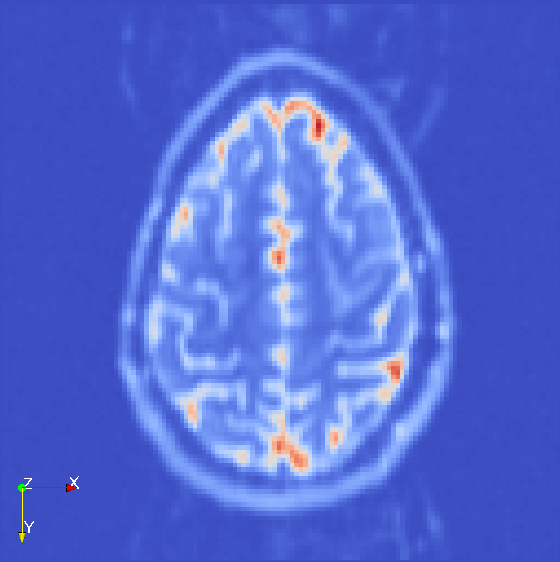
\includegraphics[height=\textwidth]{brain_ftle.PNG} a)
    \label{b)}
  \end{minipage}\hskip 15pt
  \begin{minipage}[t]{0.21\textwidth}
  \centering
  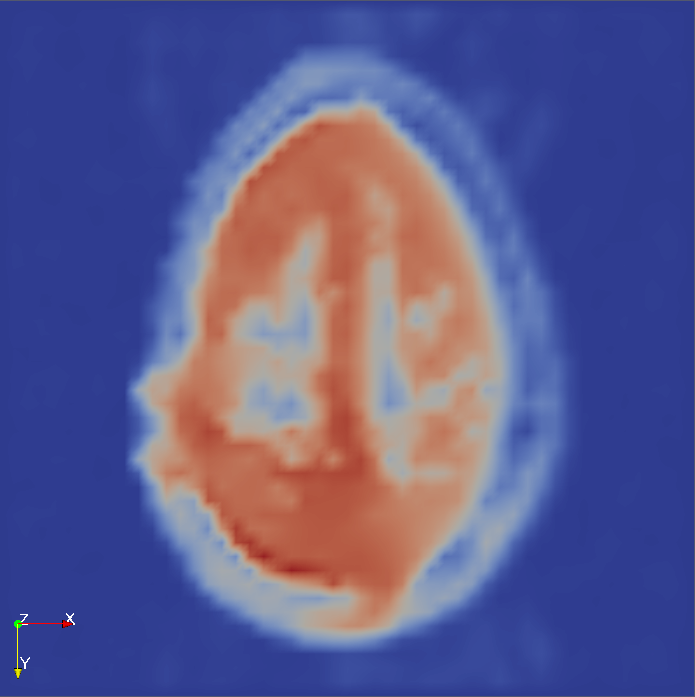
\includegraphics[height=\textwidth]{brain_surf.PNG} b)
     \label{a)}
  \end{minipage}\hskip 15pt
  \begin{minipage}[t]{0.21\textwidth}
    \centering
    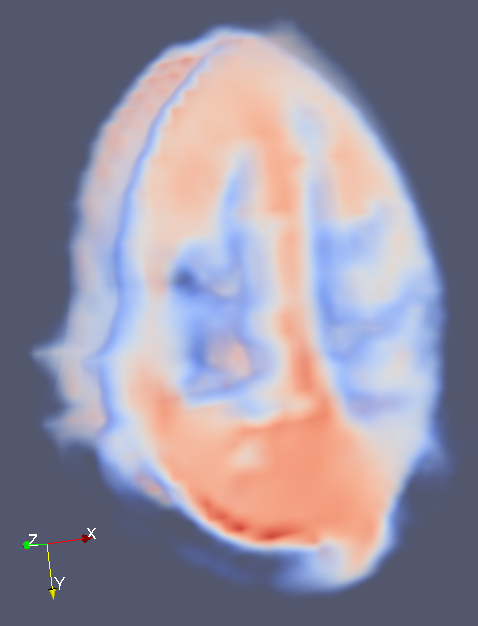
\includegraphics[height=\textwidth]{brain_volume2.PNG} \\
    c)
    \label{b)}
  \end{minipage}
  \begin{minipage}[t]{0.21\textwidth}
    \centering
    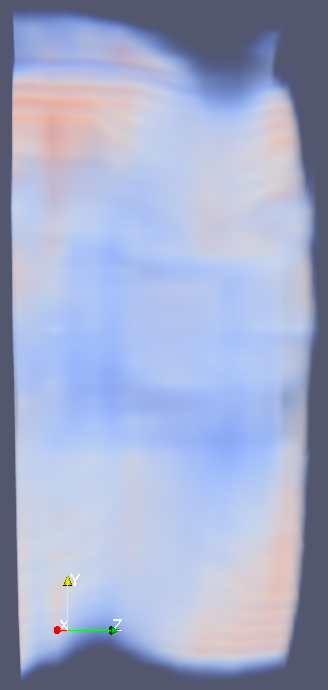
\includegraphics[height=\textwidth]{brain_cross-section.PNG} \\
    d)
    \label{b)}
  \end{minipage}
  \caption{Brain test field LTG: a) LTG($0^\circ$)-VAR1, b) LTG($0^\circ$)-VAR2, c) LTG volume, d) cross-section}
\label{brain-volumes}
\end{figure}

} % END OF FRAME

%%%%%%%%%%%%%%%%%%%%%%%%%%%%%%%%%%%%%%%%%%%%%%%%%%%%%%%%%%%%

% Alternative: put content in separate files
% Check the difference between including these files using \input{filename} and \include{filename} and see which one you like better
%\chapter{Einleitung}\label{intro}
%\input{introduction}
%
%\chapter{Voraussetzungen}\label{bg}
%\input{background}



\end{document}